% locking/locking.tex

\QuickQuizChapter{chp:Locking}{Locking}

The role of villain in much of the past few decades' concurrency research
literature is played by locking,
which stands accused of promoting deadlocks, convoying, starvation,
unfairness, data races, and all manner of other concurrency sins.
Interestingly enough, the role of workhorse in shared-memory parallel
software is played by, you guessed it, locking.

There are a number of reasons behind this dichotomy:

\begin{enumerate}
\item	Many of locking's sins have pragmatic design solutions that
	work well in most cases, for example:
	\begin{enumerate}
	\item	Lock hierarchies to avoid deadlock.
	\item	Deadlock-detection tools, for example, the Linux kernel's
		lockdep facility~\cite{JonathanCorbet2006lockdep}.
	\item	Locking-friendly data structures, such as
		arrays, hash tables, and radix trees, which will
		be covered in Chapter~\ref{chp:Data Structures}.
	\end{enumerate}
\item	Some of locking's sins are problems only at high levels of
	contention, levels reached only by poorly designed programs.
\item	Some of locking's sins are avoided by using other synchronization
	mechanisms in concert with locking.
	These other mechanisms include reference counters,
	statistical counters, simple non-blocking data structures, and RCU.
\item	Until quite recently, almost all large shared-memory parallel
	programs were developed in secret, so that it was difficult for
	most researchers to learn of these pragmatic solutions.
\item	All good stories need a villain, and locking has a long and
	honorable history serving as a research-paper whipping boy.
\end{enumerate}

This chapter will give an overview of a number of ways to avoid locking's
more serious sins.

\begin{figure}[tb]
\begin{center}
\resizebox{3in}{!}{\includegraphics{cartoons/LockingTheSlob}}
\end{center}
\caption{Locking: Villain or Slob?}
\ContributedBy{Figure}{fig:locking:Locking: Villain or Slob?}{Sarah McKenney}
\end{figure}

\begin{figure}[tb]
\begin{center}
\resizebox{3in}{!}{\includegraphics{cartoons/LockingTheHero}}
\end{center}
\caption{Locking: Workhorse or Hero?}
\ContributedBy{Figure}{fig:locking:Locking: Workhorse or Hero?}{Sarah McKenney}
\end{figure}

\section{Staying Alive}
\label{sec:locking:Staying Alive}

Given that locking stands accused of deadlock and starvation,
one important concern for shared-memory parallel developers is
simply staying alive.
The following sections therefore cover deadlock, livelock, starvation,
unfairness, and inefficiency.

\subsection{Deadlock}
\label{sec:locking:Deadlock}

Deadlock occurs when each of a group of threads is holding at least one
lock while at the same time waiting on a lock held by a member
of the same group.

Without some sort of external intervention, deadlock is forever.
No thread can acquire the lock it is waiting on until that
lock is released by the thread holding it, but the thread holding
it cannot release it until the holding thread acquires the lock that
it is waiting on.

\begin{figure}[tb]
\begin{center}
\resizebox{3in}{!}{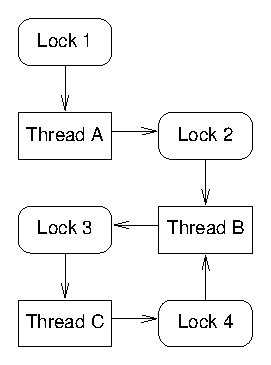
\includegraphics{locking/DeadlockCycle}}
\end{center}
\caption{Deadlock Cycle}
\label{fig:locking:Deadlock Cycle}
\end{figure}

We can create a directed-graph representation of a deadlock scenario
with nodes for threads and locks, as shown in
Figure~\ref{fig:locking:Deadlock Cycle}.
An arrow from a lock to a thread indicates that the thread holds
the lock, for example, Thread~B holds Locks~2 and 4.
An arrow from a thread to a lock indicates that the thread is waiting
on the lock, for example, Thread~B is waiting on Lock~3.

A deadlock scenario will always contain at least one deadlock cycle.
In Figure~\ref{fig:locking:Deadlock Cycle}, this cycle is
Thread~B, Lock~3, Thread~C, Lock~4, and back to Thread~B.

\QuickQuiz{}
	But the definition of deadlock only said that each thread
	was holding at least one lock and waiting on another lock
	that was held by some thread.
	How do you know that there is a cycle?
\QuickQuizAnswer{
	Suppose that there is not cycle in the graph.
	We would then have a directed acyclic graph (DAG), which would
	have at least one leaf node.

	If this leaf node was a lock, then we would have a thread
	that was waiting on a lock that wasn't held by any thread,
	which violates the definition.
	(And in this case the thread would immediately acquire the
	lock.)

	On the other hand, if this leaf node was a thread, then
	we would have a thread that was not waiting on any lock,
	again violating the definition.
	(And in this case, the thread would either be running or
	blocked on something that is not a lock.)

	Therefore, given this definition of deadlock, there must
	be a cycle in the corresponding graph.
} \QuickQuizEnd

Although there are some software environments such as database systems
that can repair an existing deadlock, this approach requires either that
one of the threads be killed or that a lock be forcibly stolen from one
of the threads.
This killing and forcible stealing can be appropriate for transactions,
but is often problematic for kernel and application-level use of locking:
dealing with the resulting partially updated structures can be extremely
complex, hazardous, and error-prone.

Kernels and applications therefore work to avoid deadlocks rather than to
recover from them.
There are a number of deadlock-avoidance strategies,
including locking hierarchies
(Section~\ref{sec:locking:Locking Hierarchies}),
local locking hierarchies
(Section~\ref{sec:locking:Local Locking Hierarchies}),
layered locking hierarchies
(Section~\ref{sec:locking:Layered Locking Hierarchies}),
strategies for dealing with APIs containing pointers to locks
(Section~\ref{sec:locking:Locking Hierarchies and Pointers to Locks}),
conditional locking
(Section~\ref{sec:locking:Conditional Locking}),
acquiring all needed locks first
(Section~\ref{sec:locking:Acquire Needed Locks First}),
single-lock-at-a-time designs
(Section~\ref{sec:locking:Single-Lock-at-a-Time Designs}),
and strategies for signal/interrupt handlers
(Section~\ref{sec:locking:Signal/Interrupt Handlers}).
Although there is no deadlock-avoidance strategy that works perfectly
for all situations, there is a good selection of deadlock-avoidance
tools to choose from.

\subsubsection{Locking Hierarchies}
\label{sec:locking:Locking Hierarchies}

Locking hierarchies order the locks and prohibit acquiring locks out
of order.
In Figure~\ref{fig:locking:Deadlock Cycle},
we might order the locks numerically, so that a thread was
forbidden from acquiring a given lock if it already held a lock
with the same or a higher number.
Thread~B has violated this hierarchy because it is attempting to
acquire Lock~3 while holding Lock~4, which permitted the deadlock
to occur.

Again, to apply a locking hierarchy, order the locks and prohibit
out-of-order lock acquisition.
In large program, it is wise to use tools to enforce your locking
hierarchy~\cite{JonathanCorbet2006lockdep}.

\begin{figure}[tbp]
{ \scriptsize
\begin{verbatim}
  1 spin_lock(&lock2);
  2 layer_2_processing(pkt);
  3 nextlayer = layer_1(pkt);
  4 spin_lock(&nextlayer->lock1);
  5 layer_1_processing(pkt);
  6 spin_unlock(&lock2);
  7 spin_unlock(&nextlayer->lock1);
\end{verbatim}
}
\caption{Protocol Layering and Deadlock}
\label{fig:locking:Protocol Layering and Deadlock}
\end{figure}

\subsubsection{Local Locking Hierarchies}
\label{sec:locking:Local Locking Hierarchies}

However, the global nature of locking hierarchies make them difficult to
apply to library functions.
After all, the program using a given library function has not even been
written yet, so how can the poor library-function implementor possibly
hope to adhere to the yet-to-be-written program's locking hierarchy?

One special case that is fortunately the common case is when
the library function does not invoke any of the caller's code.
In this case, the caller's locks will never be acquired while holding
any of the library's locks, so that there cannot be a deadlock cycle
containing locks from both the library and the caller.

\QuickQuiz{}
	Are there any exceptions to this rule, so that there really could be
	a deadlock cycle containing locks from both the library and
	the caller, even given that the library code never invokes
	any of the caller's functions?
\QuickQuizAnswer{
	Indeed there can!
	Here are a few of them:
	\begin{enumerate}
	\item	If one of the library function's arguments is a pointer
		to a lock that this library function acquires, and if
		the library function holds one if its locks while
		acquiring the caller's lock, then we could have a
		deadlock cycle involving both caller and library locks.
	\item	If one of the library functions returns a pointer to
		a lock that is acquired by the caller, and if the
		caller acquires one if its locks while holding the
		library's lock, we could again have a deadlock
		cycle involving both caller and library locks.
	\item	If one of the library functions acquires a lock and
		then returns while still holding it, and if the caller
		acquires one of its locks, we have yet another way
		to create a deadlock cycle involving both caller
		and library locks.
	\item	If the caller has a signal handler that acquires
		locks, then the deadlock cycle can involve both
		caller and library locks.
		In this case, however, the library's locks are
		innocent bystanders in the deadlock cycle.
		That said, please note that acquiring a lock from
		within a signal handler is a no-no in most
		environments---it is not just a bad idea, it
		is unsupported.
	\end{enumerate}
} \QuickQuizEnd

But suppose that a library function does invoke the caller's code.
For example, the \co{qsort()} function invokes a caller-provided
comparison function.
A concurrent implementation of \co{qsort()} likely uses locking,
which might result in deadlock in the perhaps-unlikely case where
the comparison function is a
complicated function involving locking.
How can the library function avoid deadlock?

The golden rule in this case is ``release all locks before invoking
unknown code.''
To follow this rule, the \co{qsort()} function must release all
locks before invoking the comparison function.

\QuickQuiz{}
	But if \co{qsort()} releases all its locks before invoking
	the comparison function, how can it protect against races
	with other \co{qsort()} threads?
\QuickQuizAnswer{
	By privatizing the data elements being compared
	(as discussed in Chapter~\ref{chp:Data Ownership})
	or through use of deferral mechanisms such as
	reference counting (as discussed in
	Chapter~\ref{chp:Deferred Processing}).
} \QuickQuizEnd

\begin{figure}[tb]
\begin{center}
\resizebox{3in}{!}{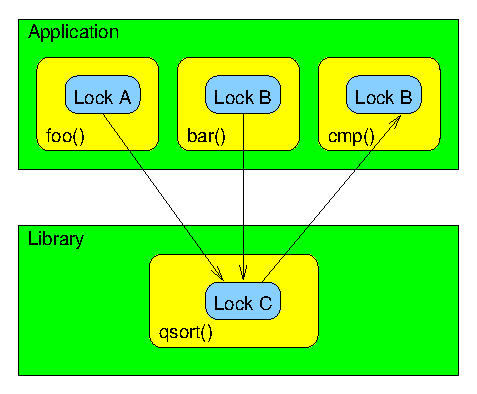
\includegraphics{locking/NonLocalLockHierarchy}}
\end{center}
\caption{Without Local Locking Hierarchy for qsort()}
\label{fig:lock:Without Local Locking Hierarchy for qsort()}
\end{figure}

\begin{figure}[tb]
\begin{center}
\resizebox{3in}{!}{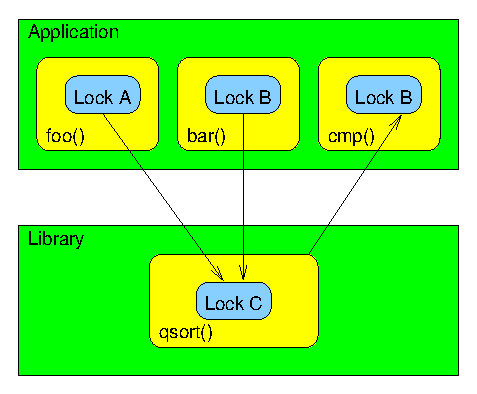
\includegraphics{locking/LocalLockHierarchy}}
\end{center}
\caption{Local Locking Hierarchy for qsort()}
\label{fig:lock:Local Locking Hierarchy for qsort()}
\end{figure}

To see the benefits of local locking hierarchies, compare
Figures~\ref{fig:lock:Without Local Locking Hierarchy for qsort()} and
\ref{fig:lock:Local Locking Hierarchy for qsort()}.
In both figures, application functions \co{foo()} and \co{bar()}
invoke \co{qsort()} while holding locks~A and B, respectively.
Because this is a parallel implementation of \co{qsort()}, it acquires
lock~C.
Function \co{foo()} passes function \co{cmp()} to \co{qsort()},
and \co{cmp()} acquires lock~B.
Function \co{bar()} passes a simple integer-comparison function (not
shown) to \co{qsort()}, and this simple function does not acquire any
locks.

Now, if \co{qsort()} holds Lock~C while calling \co{cmp()} in violation
of the golden release-all-locks rule above, as shown in
Figure~\ref{fig:lock:Without Local Locking Hierarchy for qsort()},
deadlock can occur.
To see this, suppose that one thread invokes \co{foo()} while a second
thread concurrently invokes \co{bar()}.
The first thread will acquire lock~A and the second thread will acquire
lock~B.
If the first thread's call to \co{qsort()} acquires lock~C, then it
will be unable to acquire lock~B when it calls \co{cmp()}.
But the first thread holds lock~C, so the second thread's call to
\co{qsort()} will be unable to acquire it, and thus unable to release
lock~B, resulting in deadlock.

In contrast, if \co{qsort()} releases lock~C before invoking the
comparison function (which is unknown code from \co{qsort()}'s perspective,
then deadlock is avoided as shown in
Figure~\ref{fig:lock:Local Locking Hierarchy for qsort()}.

If each module releases all locks before invoking unknown code, then
deadlock is avoided if each module separately avoids deadlock.
This rule therefore greatly simplifies deadlock analysis and greatly
improves modularity.

\subsubsection{Layered Locking Hierarchies}
\label{sec:locking:Layered Locking Hierarchies}

\begin{figure}[tb]
\begin{center}
\resizebox{3in}{!}{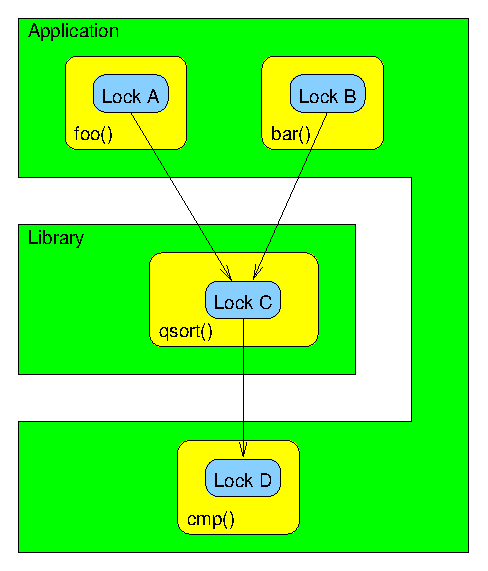
\includegraphics{locking/LayeredLockHierarchy}}
\end{center}
\caption{Layered Locking Hierarchy for qsort()}
\label{fig:lock:Layered Locking Hierarchy for qsort()}
\end{figure}

Unfortunately, it might not be possible for \co{qsort()} to release
all of its locks before invoking the comparison function.
In this case, we cannot construct a local locking hierarchy by
releasing all locks before invoking unknown code.
However, we can instead construct a layered locking hierarchy, as shown in
Figure~\ref{fig:lock:Layered Locking Hierarchy for qsort()}.
Here, the \co{cmp()} function uses a new lock~D that is acquired after
all of locks~A, B, and C, avoiding deadlock.
We therefore have three layers to the global deadlock hierarchy, the
first containing locks~A and B, the second containing lock~C, and
the third containing lock~D.

\begin{figure}[tbp]
{ \scriptsize
\begin{verbatim}
  1 struct locked_list {
  2   spinlock_t s;
  3   struct list_head h;
  4 };
  5 
  6 struct list_head *list_start(struct locked_list *lp)
  7 {
  8   spin_lock(&lp->s);
  9   return list_next(lp, &lp->h);
 10 }
 11 
 12 struct list_head *list_next(struct locked_list *lp,
 13                             struct list_head *np)
 14 {
 15   struct list_head *ret;
 16 
 17   ret = np->next;
 18   if (ret == &lp->h) {
 19     spin_unlock(&lp->s);
 20     ret = NULL;
 21   }
 22   return ret;
 23 }
\end{verbatim}
}
\caption{Concurrent List Iterator}
\label{fig:locking:Concurrent List Iterator}
\end{figure}

For another example where releasing all locks before invoking unknown
code is impractical, imagine an interator over a linked list, as shown in
Figure~\ref{fig:locking:Concurrent List Iterator} (\co{locked_list.c}).
The \co{list_start()} function acquires a lock on the list and returns
the first element (if there is one), and
\co{list_next()} either returns a pointer to the next element in the list
or releases the lock and returns \co{NULL} if the end of the list has
been reached.

\begin{figure}[tbp]
{ \scriptsize
\begin{verbatim}
  1 struct list_ints {
  2   struct list_head n;
  3   int a;
  4 };
  5 
  6 void list_print(struct locked_list *lp)
  7 {
  8   struct list_head *np;
  9   struct list_ints *ip;
 10 
 11   np = list_start(lp);
 12   while (np != NULL) {
 13     ip = list_entry(np, struct list_ints, n);
 14     printf("\t%d\n", ip->a);
 15     np = list_next(lp, np);
 16   }
 17 }
\end{verbatim}
}
\caption{Concurrent List Iterator Usage}
\label{fig:locking:Concurrent List Iterator Usage}
\end{figure}

Figure~\ref{fig:locking:Concurrent List Iterator Usage} shows how
this list iterator may be used.
Lines~1-4 define the \co{list_ints} element containing a single integer,
and lines~6-17 show how to iterate over the list.
Line~11 locks the list and fetches a pointer to the first element,
line~13 provides a pointer to our enclosing \co{list_ints} structure,
line~14 prints the corresponding integer, and
line~15 moves to the next element.
This is quite simple, and hides all of the locking.

That is, the locking remains hidden as long as the code processing each
list element does not itself acquire a lock that is held across some
other call to \co{list_start()} or \co{list_next()}, which results in
deadlock.
We can avoid the deadlock by layering the locking hierarchy
to take the list-iterator locking into account.

This layered approach can be extended to an arbitrarily large number of layers,
but each added layer increases the complexity of the locking design.
Such increases in complexity are particularly inconvenient for some
types of object-oriented designs, in which control passes back and forth
among a large group of objects in an undisciplined manner.
This mismatch between the habits of object-oriented design and the
need to avoid deadlock is an important reason why parallel programming
is perceived by some to be so difficult.

Some alternatives to highly layered locking hierarchies are covered in
Chapter~\ref{chp:Deferred Processing}.

\subsubsection{Locking Hierarchies and Pointers to Locks}
\label{sec:locking:Locking Hierarchies and Pointers to Locks}

Althought there are some exceptions, an external API containing a pointer
to a lock is very often a misdesigned API.
Handing an internal lock to some other software component is after all
the antithesis of information hiding, which is in turn a key design
principle.

\QuickQuiz{}
	Name one common exception where it is perfectly reasonable
	to pass a pointer to a lock into a function.
\QuickQuizAnswer{
	Locking primitives, of course!
} \QuickQuizEnd

One exception is functions that hand off some entity,
where the caller's lock must be held until the handoff is complete,
but where the lock must be released before the function returns.
One example of such a function is the POSIX \co{pthread_cond_wait()}
function, where passing an pointer to a \co{pthread_mutex_t}
prevents hangs due to lost wakeups.

\QuickQuiz{}
	Doesn't the fact that \co{pthread_cond_wait()} first releases the
	mutex and then re-acquires it eliminate the possibility of deadlock?
\QuickQuizAnswer{
	Absolutely not!

	Consider the a program that acquires \co{mutex_a}, and then
	\co{mutex_b}, in that order, and then passes \co{mutex_a}
	to \co{pthread_cond_wait}.
	Now, \co{pthread_cond_wait} will release \co{mutex_a}, but
	will re-acquire it before returning.
	If some other thread acquires \co{mutex_a} in the meantime
	and then blocks on \co{mutex_b}, the program will deadlock.
} \QuickQuizEnd

In short, if you find yourself exporting an API with a pointer to a
lock as an argument or the return value, do youself a favor and carefully
reconsider your API design.
It might well be the right thing to do, but experience indicates that
this is unlikely.

\subsubsection{Conditional Locking}
\label{sec:locking:Conditional Locking}

But suppose that there is no reasonable locking hierarchy.
This can happen in real life, for example, in layered network protocol stacks
where packets flow in both directions.
In the networking case, it might be necessary to hold the locks from
both layers when passing a packet from one layer to another.
Given that packets travel both up and down the protocol stack, this
is an excellent recipe for deadlock, as illustrated in
Figure~\ref{fig:locking:Protocol Layering and Deadlock}.
Here, a packet moving down the stack towards the wire must acquire
the next layer's lock out of order.
Given that packets moving up the stack away from the wire are acquiring
the locks in order, the lock acquisition in line~4 of the figure
can result in deadlock.

\begin{figure}[tbp]
{ \scriptsize
\begin{verbatim}
  1 retry:
  2   spin_lock(&lock2);
  3   layer_2_processing(pkt);
  4   nextlayer = layer_1(pkt);
  5   if (!spin_trylock(&nextlayer->lock1)) {
  6     spin_unlock(&lock2);
  7     spin_lock(&nextlayer->lock1);
  8     spin_lock((&lock2);
  9     if (layer_1(pkt) != nextlayer) {
 10       spin_unlock(&nextlayer->lock1);
 11       spin_unlock((&lock2);
 12       goto retry;
 13     }
 14   }
 15   layer_1_processing(pkt);
 16 spin_unlock(&lock2);
 17 spin_unlock(&nextlayer->lock1);
\end{verbatim}
}
\caption{Avoiding Deadlock Via Conditional Locking}
\label{fig:locking:Avoiding Deadlock Via Conditional Locking}
\end{figure}

One way to avoid deadlocks in this case is to impose a locking hierarchy,
but when it is necessary to acquire a lock out of order, acquire it
conditionally, as shown in
Figure~\ref{fig:locking:Avoiding Deadlock Via Conditional Locking}.
Instead of unconditionally acquiring the layer-1 lock, line~5
conditionally acquires the lock using the \co{spin_trylock()} primitive.
This primitive acquires the lock immediately if the lock is available
(returning non-zero), and otherwise returns zero without acquiring the lock.

If \co{spin_trylock()} was successful, line~15 does the needed
layer-1 processing.
Otherwise, line~6 releases the lock, and lines~7 and 8 acquire them in
the correct order.
Unfortunately, there might be multiple networking devices on
the system (e.g., Ethernet and WiFi), so that the \co{layer_1()}
function must make a routing decision.
This decision might change at any time, especially if the system
is mobile.\footnote{
	And, in contrast to the 1900s, mobility is the common case.}
Therefore, line~9 must recheck the decision, and if it has changed,
must release the locks and start over.

\QuickQuiz{}
	Can the transformation from
	Figure~\ref{fig:locking:Protocol Layering and Deadlock} to
	Figure~\ref{fig:locking:Avoiding Deadlock Via Conditional Locking}
	be applied universally?
\QuickQuizAnswer{
	Absolutely not!

	This transformation assumes that the
	\co{layer_2_processing()} function is idempotent, given that
	it might be executed multiple times on the same packet when
	the \co{layer_1()} routing decision changes.
	Therefore, in real life, this transformation can become
	arbitrarily complex.
} \QuickQuizEnd

\QuickQuiz{}
	But the complexity in
	Figure~\ref{fig:locking:Avoiding Deadlock Via Conditional Locking}
	is well worthwhile given that it avoids deadlock, right?
\QuickQuizAnswer{
	Maybe.

	If the routing decision in \co{layer_1()} changes often enough,
	the code will always retry, never making forward progress.
	This is termed ``livelock'' if no thread makes any forward progress or
	``starvation''
	if some threads make forward progress but other do not
	(see Section~\ref{sec:locking:Livelock and Starvation}).
} \QuickQuizEnd

\subsubsection{Acquire Needed Locks First}
\label{sec:locking:Acquire Needed Locks First}

In an important special case of conditional locking all needed
locks are acquired before any processing is carried out.
In this case, processing need not be idempotent: if it turns out
to be impossible to acquire a given lock without first releasing
one that was already acquired, just release all the locks and
try again.
Only once all needed locks are held will any processing be carried out.

However, this procedure can result in \emph{livelock}, which will
be discussed in
Section~\ref{sec:locking:Livelock and Starvation}.

\subsubsection{Single-Lock-at-a-Time Designs}
\label{sec:locking:Single-Lock-at-a-Time Designs}

In some cases, it is possible to avoid nesting locks, thus avoiding
deadlock.
For example, if a problem is perfectly partitionable, a single
lock may be assigned to each partition.
Then a thread working on a given partition need only acquire the one
corresponding lock.
Because no thread ever holds more than one lock at a time,
deadlock is impossible.

However, there must be some mechanism to ensure that the needed data
structures remain in existence during the time that neither lock is
held.
One such mechanism is discussed in
Section~\ref{sec:locking:Lock-Based Existence Guarantees}
and several others are presented in
Chapter~\ref{chp:Deferred Processing}.

\subsubsection{Signal/Interrupt Handlers}
\label{sec:locking:Signal/Interrupt Handlers}

Deadlocks involving signal handlers are often quickly dismissed by
noting that it is not legal to invoke \co{pthread_mutex_lock()} from
within a signal handler~\cite{OpenGroup1997pthreads}.
However, it is possible (though almost always unwise) to hand-craft
locking primitives that can be invoked from signal handlers.
Besides which, almost all operating-system kernels permit locks to
be acquired from within interrupt handlers, which are the kernel analog
to signal handlers.

The trick is to block signals (or disable interrupts, as the case may be)
when acquiring any lock that might be acquired within an interrupt
handler.
Furthermore, if holding such a lock, it is illegal to attempt to
acquire any lock that is every acquired without block signals
outside of a signal handler.

If a lock is acquired by the handlers for several signals, then each
and every one of these signals must be blocked whenever that lock is
acquired, even when that
lock is acquired within a signal handler.

\QuickQuiz{}
	How can you legally block signals within a signal handler?
\QuickQuizAnswer{
	One of the simplest and fastest ways to do so is to use
	the \co{sa_mask} field of the \co{struct sigaction} that
	you pass to \co{sigaction()} when setting up the signal.
} \QuickQuizEnd

Unfortunately, blocking and unblocking signals can be expensive in
some operating systems, notably including Linux, so performance
concerns often mean that locks acquired in signal handlers are only
acquired in signal handlers, and that lockless synchronization
mechanisms are used to communicate between application code and
signal handlers.

Or that signal handlers are avoided completely except for handling
fatal errors.

\subsubsection{Discussion}
\label{sec:locking:Locking Hierarchy Discussion}

There are a large number of deadlock-avoidance strategies available to
the shared-memory parallel programmer, but there are sequential
programs for which none of them is a good fit.
This is one of the reasons that expert programmers have more than
one tool in their toolbox: locking is a powerful concurrency
tool, but there are jobs better addressed with other tools.

\QuickQuiz{}
	Given an object-oriented application that passes control freely
	among a group of objects such that there is no reasonable
	locking hierarchy, layered or otherwise, how can this
	application be parallelized?
\QuickQuizAnswer{
	There are a number of approaches:
	\begin{enumerate}
	\item	In the case of parametric search via simulation,
		where a large number of simulations will be run
		in order to converge on (for example) a good design
		for a mechanical or electrical device, leave the
		simulation single-threaded, but run many of them
		in parallel.
		This retains the object-oriented design, and
		gains parallelism at a higher level.
	\item	Partition the objects into groups such that there
		is no need for a given to operate on objects in
		more than one group at a given time.
		Then associate a lock with each group.
		This is an example of a single-lock-at-a-time
		design, which discussed in
		Section~\ref{sec:locking:Single-Lock-at-a-Time Designs}.
	\item	Partition the objects into groups such that threads
		can all operate on objects in the groups in some
		groupwise ordering.
		Then associate a lock with each group, and impose a
		locking hierarchy over the groups.
	\item	Impose an arbitrarily selected hierarchy on the locks,
		and then use conditional locking if it is necessary
		to acquire a lock out of order, as was discussed in
		Section~\ref{sec:locking:Conditional Locking}.
	\item	Before carrying out a given group of operations, predict
		which locks will be acquired, and attempt to acquire them
		before actually carrying out any updates.
		This approach was discussed in
		Section~\ref{sec:locking:Acquire Needed Locks First}.
	\item	Use transactional memory.
		This approach has a number of advantages and disadvantages
		which will be discussed in
		Section~\ref{sec:future:Transactional Memory}.
	\item	Refactor the application to be more concurrency-friendly.
		This would likely also have the side effect of making
		the application run faster single-threaded, but might
		also make it more difficult to modify the application
		when needed to account for changing conditions and
		requirements.
	\item	Use techniques from later chapters in addition to locking.
	\end{enumerate}
} \QuickQuizEnd

Nevertheless, the strategies described in this section have proven
quite useful in many settings.

\subsection{Livelock and Starvation}
\label{sec:locking:Livelock and Starvation}

\begin{figure}[tbp]
{ \scriptsize
\begin{verbatim}
  1 void thread1(void)
  2 {
  3 retry:
  4   spin_lock(&lock1);
  5   do_one_thing();
  6   if (!spin_trylock(&lock2)) {
  7     spin_unlock(&lock1);
  8     goto retry;
  9   }
 10   do_another_thing();
 11   spin_unlock(&lock2);
 12   spin_unlock(&lock1);
 13 }
 14 
 15 void thread2(void)
 16 {
 17 retry:
 18   spin_lock(&lock2);
 19   do_a_third_thing();
 20   if (!spin_trylock(&lock1)) {
 21     spin_unlock(&lock2);
 22     goto retry;
 23   }
 24   do_a_fourth_thing();
 25   spin_unlock(&lock1);
 26   spin_unlock(&lock2);
 27 }
\end{verbatim}
}
\caption{Abusing Conditional Locking}
\label{fig:locking:Abusing Conditional Locking}
\end{figure}

Although conditional locking can be an effective deadlock-avoidance
mechanism, it can be abused.
Consider for example the beautifully symmetric example shown in
Figure~\ref{fig:locking:Abusing Conditional Locking}.
This example's beauty hides an ugly livelock.
To see this, consider the following sequence of events:

\begin{enumerate}
\item	Thread~1 acquires \co{lock1} on line~4, then invokes
	\co{do_one_thing()}.
\item	Thread~2 acquires \co{lock2} on line~18, then invokes
	\co{do_a_third_thing()}.
\item	Thread~1 attempts to acquire \co{lock2}, but fails because
	Thread~2 holds it.
\item	Thread~2 attempts to acquire \co{lock1}, but fails because
	Thread~1 holds it.
\item	Thread~1 releases \co{lock1}, and jumps to \co{retry}.
\item	Thread~2 releases \co{lock2}, and jumps to \co{retry}.
\item	The livelock dance repeats from the beginning.
\end{enumerate}

\QuickQuiz{}
	How can the livelock shown in
	Figure~\ref{fig:locking:Abusing Conditional Locking}
	be avoided?
\QuickQuizAnswer{
	This is left as an exercise to the reader.
	Figure~\ref{fig:locking:Avoiding Deadlock Via Conditional Locking}
	provides some good hints.
	In many cases, livelocks are a hint that you should revisit your
	locking design.
	Or visit it in the first place if your locking design
	``just grew''.
} \QuickQuizEnd

Starvation is very similar to livelock.
Put another way, livelock is an extreme form of starvation where
a group of threads starve, rather than just one of them.\footnote{
	Try not to get too hung up on the exact definitions of terms
	like livelock, starvation, and unfairness.
	Anything that causes a group of threads to fail to make good
	forward progress is a problem that needs to be fixed, regardless
	of what name you choose for it.}

\begin{figure}[tbp]
{ \scriptsize
\begin{verbatim}
  1 void thread1(void)
  2 {
  3   unsigned int wait = 1;
  4 retry:
  5   spin_lock(&lock1);
  6   do_one_thing();
  7   if (!spin_trylock(&lock2)) {
  8     spin_unlock(&lock1);
  9     sleep(wait);
 10     wait = wait << 1;
 11     goto retry;
 12   }
 13   do_another_thing();
 14   spin_unlock(&lock2);
 15   spin_unlock(&lock1);
 16 }
 17 
 18 void thread2(void)
 19 {
 20   unsigned int wait = 1;
 21 retry:
 22   spin_lock(&lock2);
 23   do_a_third_thing();
 24   if (!spin_trylock(&lock1)) {
 25     spin_unlock(&lock2);
 26     sleep(wait);
 27     wait = wait << 1;
 28     goto retry;
 29   }
 30   do_a_fourth_thing();
 31   spin_unlock(&lock1);
 32   spin_unlock(&lock2);
 33 }
\end{verbatim}
}
\caption{Conditional Locking and Exponential Backoff}
\label{fig:locking:Conditional Locking and Exponential Backoff}
\end{figure}

Livelock and starvation are serious issues in software transactional
memory implementations, and so the concept of \emph{contention
manager} has been introduced to encapsulate these issues.
In the case of locking, simple exponential backoff can often address
livelock and starvation.
The idea is to introduce exponentially increasing delays before each
retry, as shown in
Figure~\ref{fig:locking:Conditional Locking and Exponential Backoff}.

\QuickQuiz{}
	What problems can you spot in the code in
	Figure~\ref{fig:locking:Conditional Locking and Exponential Backoff}?
\QuickQuizAnswer{
	Here are a couple:
	\begin{enumerate}
	\item	A one-second wait is way too long for most uses.
		Wait intervals should begin with roughly the time
		required to execute the critical section, which will
		normally be in the microsecond or millisecond range.
	\item	The code does not check for overflow.
		On the other hand, this bug is nullified 
		by the previous bug: 32 bits worth of seconds is
		more than 50 years.
	\end{enumerate}
} \QuickQuizEnd

\subsection{Unfairness}
\label{sec:locking:Unfairness}

\begin{figure}[tb]
\begin{center}
\resizebox{3in}{!}{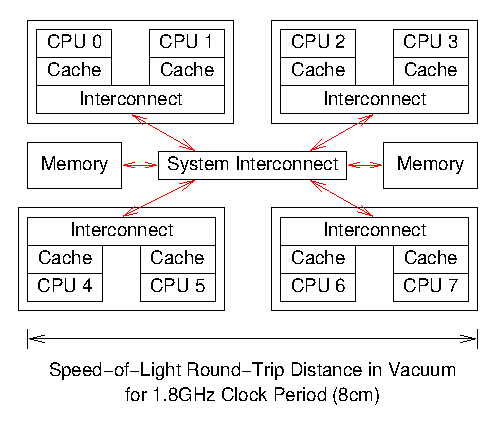
\includegraphics{cpu/SystemArch}}
\end{center}
\caption{System Architecture and Lock Unfairness}
\label{fig:lock:System Architecture and Lock Unfairness}
\end{figure}

Unfairness can be thought of as a less-severe form of starvation,
where a subset of threads contending for a given lock are granted
the lion's share of the acquisitions.
This can happen on machines with shared caches or NUMA characteristics,
for example, as shown in
Figure~\ref{fig:lock:System Architecture and Lock Unfairness}.
If CPU~0 releases a lock that all the other CPUs are attempting
to acquire, the interconnect shared between CPUs~0 and 1 means that
CPU~1 will have an advantage over CPUs~2-7.
Therefore CPU~1 will likely acquire the lock.
If CPU~1 hold the lock long enough for CPU~0 to be requesting the
lock by the time CPU~1 releases it and vice versa, the lock can
shuttle between CPUs~1 and 2, bypassing CPUs~2-7.

Of course, if the lock contention is so high, you should take it as
a hint to revisit your locking design.
Given a more reasonable level of lock contention, there would be
frequent periods when the lock was not held at all, which would
prevent unfairness altogether.

\QuickQuiz{}
	Wouldn't it be better just to use a good parallel design
	so that lock contention was low enough to avoid unfairness?
\QuickQuizAnswer{
	It would be better in some sense, but there are situations
	where it can be appropriate to use
	designs that sometimes result in high lock contentions.

	For example, imagine a system that is subject to a rare error
	condition.
	It might well be best to have a simple error-handling design
	that has poor performance and scalability for the duration of
	the rare error condition, as opposed to a complex and
	difficult-to-debug design that is helpful only when one of
	those rare error conditions is in effect.

	That said, it is usually worth putting some effort into
	attempting to produce a design that both simple as well as
	efficient during error condsitions, for example by partitioning
	the problem.
} \QuickQuizEnd

\subsection{Inefficiency}
\label{sec:locking:Inefficiency}

Locks are implemented using atomic instructions and memory barriers,
and often involve cache misses.
As we saw in Chapter~\ref{chp:Hardware and its Habits},
these instructions are quite expensive, roughly two
orders of magnitude greater overhead than simple instructions.
This can be a serious problem for locking: If you protect a single
instruction with a lock, you will increase the overhead by a factor
of one hundred.
Even assuming perfect scalability, \emph{one hundred} CPUs would
be required to keep up with a single CPU executing the same code
without locking.

This situation underscores the synchronization-granularity
tradeoff discussed in Section~\ref{sec:SMPdesign:Synchronization Granularity},
especially Figure~\ref{fig:SMPdesign:Synchronization Efficiency}:
Too coarse a granularity will limit scalability, while too fine a
granularity will result in excessive synchronization overhead.

That said, once a lock is held, the data protected by that lock can
be accessed by the lock holder without interference.
Acquiring a lock might be expensive, but once held, the CPU's caches
are an effective performance booster, at least for large critical sections.

\QuickQuiz{}
	How might the lock holder be interfered with?
\QuickQuizAnswer{
	If the data protected by the lock is in the same cache line
	as the lock itself, then attempts by other CPUs to acquire
	the lock will result in expensive cache misses on the part
	of the CPU holding the lock.
	In contrast, if the lock is in a different cache line than
	the data that it protects, the CPU holding the lock will
	usually suffer a cache miss only on first access to a given
	variable.
	This is a special case of false sharing, which can also occur
	if a pair of variables protected by different locks happen
	to share a cache line.
} \QuickQuizEnd

\section{Types of Locks}
\label{sec:locking:Types of Locks}

There are a surprising number of types of locks, more than this
short chapter can possibly do justice to.
The following sections discuss
exclusive locks (Section~\ref{sec:locking:Exclusive Locks}),
reader-writer locks (Section~\ref{sec:locking:Reader-Writer Locks}), and
multi-role locks (Section~\ref{sec:locking:Beyond Reader-Writer Locks}).

\subsection{Exclusive Locks}
\label{sec:locking:Exclusive Locks}

Exclusive locks are what they say they are: only one thread may hold
the lock at a time.
The holder of such a lock thus has exclusive access to all data protected
by that lock, hence the name.

Of course, this all assumes that this lock is held across all accesses
to data purportedly protected by the lock.
Although there are some tools that can help, the ultimate responsibility
for ensuring that the lock is acquired in all necessary code paths
rests with the developer.

\subsection{Reader-Writer Locks}
\label{sec:locking:Reader-Writer Locks}

Reader-writer locks~\cite{Courtois71}
permit any number of readers to hold the lock
concurrently on the one hand or a single writer to hold the lock
on the other.
In theory, then, reader-writer locks should allow excellent scalability
for data that is read often and written rarely.
In practice, the scalability will depend on the reader-writer lock
implementation.

The classic reader-writer lock implementation involves a set of
counters and flags that are manipulated atomically.
This type of implementation suffers from the same problem as does
exclusive locking for short critical sections: The overhead of acquiring
and releasing the lock
is about two orders of magnitude greater than the overhead
of a simple instruction.
Of course, if the critical section is long enough, the overhead of
acquiring and releasing the lock becomes negligible.
However, because only
one thread at a time can be manipulating the lock, the required
critical-section size increases with the number of CPUs.

It is possible to design a reader-writer lock that is much more
favorable to readers through use of per-thread exclusive
locks~\cite{WilsonCHsieh92a}.
To read, a thread acquires only its own lock.
To write, a thread acquires all locks.
In the absence of writers, each reader incurs only atomic-instruction
and memory-barrier overhead, with no cache misses, which is quite
good for a locking primitive.
Unfortunately, writers must incur cache misses as well as atomic-instruction
and memory-barrier overhead---multiplied by the number of threads.

In short, reader-writer locks can be quite useful in a number of
situations, but each type of implementation does have its drawbacks.

\subsection{Beyond Reader-Writer Locks}
\label{sec:locking:Beyond Reader-Writer Locks}

\begin{table}
\small
\begin{center}
\begin{tabular}{l||c|c|c|c|c|c}
	~ ~ ~ ~ ~ ~ ~ ~ ~
	& \begin{picture}(6,70)(0,0)
		\rotatebox{90}{Null (Not Held)}
	  \end{picture}
	& \begin{picture}(6,70)(0,0)
		\rotatebox{90}{Concurrent Read}
	  \end{picture}
	& \begin{picture}(6,70)(0,0)
		\rotatebox{90}{Concurrent Write}
	  \end{picture}
	& \begin{picture}(6,70)(0,0)
		\rotatebox{90}{Protected Read}
	  \end{picture}
	& \begin{picture}(6,70)(0,0)
		\rotatebox{90}{Protected Write}
	  \end{picture}
	& \begin{picture}(6,70)(0,0)
		\rotatebox{90}{Exclusive}
	  \end{picture}
	\\
	\hline
%				 NL  CR  CW  PR    PW  EX
	\hline
	Null (Not Held)		& ~ & ~ & ~   & ~ & ~ & ~ \\
	\hline
	Concurrent Read		& ~ & ~ & ~   & ~ & ~ & X \\
	\hline
	Concurrent Write	& ~ & ~ & ~   & X & X & X \\
	\hline
	Protected Read		& ~ & ~ & X   & ~ & X & X \\
	\hline
	Protected Write		& ~ & ~ & X   & X & X & X \\
	\hline
	Exclusive		& ~ & X & X   & X & X & X \\
\end{tabular}
\end{center}
\caption{VAX/VMS Distributed Lock Manager Policy}
\label{tab:locking:VAX/VMS Distributed Lock Manager Policy}
\end{table}

Reader-writer locks and exclusive locks differ in their admission
policy: exclusive locks allow at most one holder, while reader-writer
locks permit an arbitrary number of read-holders (but only one write-holder).
There is a very large number of possible admission policies, one of
the more elaborate being that of the VAX/VMS distributed lock
manager (DLM)~\cite{Snaman87}, which is shown in
Table~\ref{tab:locking:VAX/VMS Distributed Lock Manager Policy}.
Blank cells indicate compatible modes, while cells containing ``X''
indicate incompatible modes.

The VAX/VMS DLM uses six modes.
For purposes of comparison, exclusive
locks use two modes (not held and held), while reader-writer locks
use three modes (not held, read held, and write held).

The first mode is null, or not held.
This mode is compatible with all other modes, which is to be expected:
If a thread is not holding a lock, it should not prevent any
other thread from acquiring that lock.

The second mode is concurrent read, which is compatible with every other
mode except for exclusive.
The concurrent-read mode might be used to accumulate approximate
statistics on a data structure, while permitting updates to proceed
concurrently.

The third mode is concurrent write, which is compatible with null,
concurrent read, and concurrent write.
The concurrent-write mode might be used to update approximate statistics,
while still permitting reads and concurrent updates to proceed
concurrently.

The fourth mode is protected read, which is compatible with null,
concurrent read, and protected read.
The protected-read mode might be used to obtain a consistent snapshot
of the data structure, while permitting reads but not updates to
proceed concurrently.

The fifth mode is protected write, which is compatible with null and
protected read.
The protected-write mode might be used to carry out updates to a data
structure that could interfere with protected readers but which could
be tolerated by concurrent readers.

The sixth and final mode is exclusive, which is compatible only with null.
The exclusive mode is used when it is necessary to exclude all other accesses.

It is interesting to note that exclusive locks and reader-writer locks
can be emulated by the VAX/VMS DLM.
Exclusive locks would use only the null and exclusive modes, while
reader-writer locks might use the null, protected-read, and
protected-write modes.

\QuickQuiz{}
	Is there any other way for the VAX/VMS DLM to emulate
	a reader-writer lock?
\QuickQuizAnswer{
	There are in fact several.
	One way would be to use the null, protected-read, and exclusive
	modes.
	Another way would be to use the null, protected-read, and
	concurrent-write modes.
	A third way would be to use the null, concurrent-read, and
	exclusive modes.
} \QuickQuizEnd

Although the VAX/VMS DLM policy has seen widespread production use
for distributed databases, it does not appear to be used much in
shared-memory applications.
One possible reason for this is that the greater communication overheads
of distributed databases can hide the greater overhead of the
VAX/VMS DLM's more-complex admission policy.

Nevertheless, the VAX/VMS DLM is an interesting illustration of just
how flexible the concepts behind locking can be.

% locking-existence.tex

\section{Lock-Based Existence Guarantees}
\label{sec:locking:Lock-Based Existence Guarantees}

{ \scriptsize
\begin{verbbox}
  1 int delete(int key)
  2 {
  3   int b;
  4   struct element *p;
  5
  6   b = hashfunction(key);
  7   p = hashtable[b];
  8   if (p == NULL || p->key != key)
  9     return 0;
 10   spin_lock(&p->lock);
 11   hashtable[b] = NULL;
 12   spin_unlock(&p->lock);
 13   kfree(p);
 14   return 1;
 15 }
\end{verbbox}
}
\begin{figure}[tbp]
\centering
\theverbbox
\caption{Per-Element Locking Without Existence Guarantees}
\label{fig:locking:Per-Element Locking Without Existence Guarantees}
\end{figure}

A key challenge in parallel programming is to provide
\emph{existence guarantees}~\cite{Gamsa99},
so that attempts to access a given object can rely on that object
being in existence throughout a given access attempt.
In some cases, existence guarantees are implicit:

\begin{enumerate}
\item	Global variables and static local variables in the base module
	will exist as long as the application is running.
\item	Global variables and static local variables in a loaded module
	will exist as long as that module remains loaded.
\item	A module will remain loaded as long as at least one of its functions
	has an active instance.
\item	A given function instance's on-stack variables will exist until
	that instance returns.
\item	If you are executing within a given function or have been
	called (directly or indirectly) from that function,
	then the given function has an active instance.
\end{enumerate}

These implicit existence guarantees are straightforward, though
bugs involving implicit existence guarantees really can happen.

\QuickQuiz{}
	How can relying on implicit existence guarantees result in
	a bug?
\QuickQuizAnswer{
	Here are some bugs resulting from improper use of implicit
	existence guarantees:
	\begin{enumerate}
	\item	A program writes the address of a global variable to
		a file, then a later instance of that same program
		reads that address and attempts to dereference it.
		This can fail due to address-space randomization,
		to say nothing of recompilation of the program.
	\item	A module can record the address of one of its variables
		in a pointer located in some other module, then attempt
		to dereference that pointer after the module has
		been unloaded.
	\item	A function can record the address of one of its on-stack
		variables into a global pointer, which some other
		function might attempt to dereference after that function
		has returned.
	\end{enumerate}
	I am sure that you can come up with additional possibilities.
} \QuickQuizEnd

But the more interesting---and troublesome---guarantee involves
heap memory: A dynamically allocated data structure will exist until it
is freed.
The problem to be solved is to synchronize the freeing of the structure
with concurrent accesses to that same structure.
One way to do this is with \emph{explicit guarantees}, such as locking.
If a given structure may only be freed while holding a given lock, then holding
that lock guarantees that structure's existence.

But this guarantee depends on the existence of the lock itself.
One straightforward way to guarantee the lock's existence is to
place the lock in a global variable, but global locking has the disadvantage
of limiting scalability.
One way of providing scalability that improves as the size of the
data structure increases is to place a lock in each element of the
structure.
Unfortunately, putting the lock that is to protect a data element
in the data element itself is subject to subtle race conditions,
as shown in
Figure~\ref{fig:locking:Per-Element Locking Without Existence Guarantees}.

\QuickQuiz{}
	What if the element we need to delete is not the first element
	of the list on line~8 of
	Figure~\ref{fig:locking:Per-Element Locking Without Existence Guarantees}?
\QuickQuizAnswer{
	This is a very simple hash table with no chaining, so the only
	element in a given bucket is the first element.
	The reader is invited to adapt this example to a hash table with
	full chaining.
} \QuickQuizEnd

\QuickQuiz{}
	What race condition can occur in
	Figure~\ref{fig:locking:Per-Element Locking Without Existence Guarantees}?
\QuickQuizAnswer{
	Consider the following sequence of events:
	\begin{enumerate}
	\item	Thread~0 invokes \co{delete(0)}, and reaches line~10 of
		the figure, acquiring the lock.
	\item	Thread~1 concurrently invokes \co{delete(0)}, reaching
		line~10, but spins on the lock because Thread~0 holds it.
	\item	Thread~0 executes lines~11-14, removing the element from
		the hashtable, releasing the lock, and then freeing the
		element.
	\item	Thread~0 continues execution, and allocates memory, getting
		the exact block of memory that it just freed.
	\item	Thread~0 then initializes this block of memory as some
		other type of structure.
	\item	Thread~1's \co{spin_lock()} operation fails due to the
		fact that what it believes to be \co{p->lock} is no longer
		a spinlock.
	\end{enumerate}
	Because there is no existence guarantee, the identity of the
	data element can change while a thread is attempting to acquire
	that element's lock on line~10!
} \QuickQuizEnd

{ \scriptsize
\begin{verbbox}
  1 int delete(int key)
  2 {
  3   int b;
  4   struct element *p;
  5   spinlock_t *sp;
  6
  7   b = hashfunction(key);
  8   sp = &locktable[b];
  9   spin_lock(sp);
 10   p = hashtable[b];
 11   if (p == NULL || p->key != key) {
 12     spin_unlock(sp);
 13     return 0;
 14   }
 15   hashtable[b] = NULL;
 16   spin_unlock(sp);
 17   kfree(p);
 18   return 1;
 19 }
\end{verbbox}
}
\begin{figure}[tbp]
\centering
\theverbbox
\caption{Per-Element Locking With Lock-Based Existence Guarantees}
\label{fig:locking:Per-Element Locking With Lock-Based Existence Guarantees}
\end{figure}

One way to fix this example is to use a hashed set of global locks, so
that each hash bucket has its own lock, as shown in
Figure~\ref{fig:locking:Per-Element Locking With Lock-Based Existence Guarantees}.
This approach allows acquiring the proper lock (on line~9) before
gaining a pointer to the data element (on line~10).
Although this approach works quite well for elements contained in a
single partitionable data structure such as the hash table shown in the
figure, it can be problematic if a given data element can be a member
of multiple hash tables or given more-complex data structures such
as trees or graphs.
These problems can be solved, in fact, such solutions form the basis
of lock-based software transactional memory
implementations~\cite{Shavit95,DaveDice2006DISC}.
However,
Chapter~\ref{chp:Deferred Processing}
describes simpler---and faster---ways of providing existence guarantees.


\section{Locking: Hero or Villain?}

As is often the case in real life, locking can be either hero or villain,
depending on how it is used and on the problem at hand.
Locking is perhaps the most widely used and most generally useful tool,
but it should not be the only tool in your parallel-programming toolbox.

The next few chapters will discuss other tools, and how they can best
be used in concert with locking and with each other.
